%
% teil3.tex -- Beispiel-File für Teil 3
%
% (c) 2020 Prof Dr Andreas Müller, Hochschule Rapperswil
%
% !TEX root = ../../buch.tex
% !TEX encoding = UTF-8
%
\subsection{Termination
\label{genetic_algorithm:termination}}
Der Startpunkt des genetischen Algorithmus ist die Initialisierung.
Dabei wird eine zufällige Population von möglichen Lösungen erstellt.
Diese wird als ein genetischer String dargestellt.

\begin{figure} [h]
	\centering
	
\includegraphics[width=0.8\textwidth]{
        papers/variationsprinzip_algorithmen/images/teil2/01_genetic_string.png
        }
	\caption{Beispiel von möglichen Genetic String}
	\label{fig:possible_genetic_string}
\end{figure}

Dabei wird in jeder Position das Gen aktiviert mit 1 oder deaktiviert mit 0.
Problematik für Stätte funktioniert dies nicht, da wir eine Stadt nicht
einfach aus oder anschalten können. Beim Gen wie oben ändert sich die funktioniert
an der Position nicht. Beispiel Feld 2 ist veranwortlich, dass die Farbe Grün
dargestellt wird. Bei den Städten ändert sich aber die Reihenfolge, da wird 
nicht einfach Ein oder ausgeschaltet. Zur einfachheit wird in den Stellen 
die Nummer der Stadt genommen.

\begin{figure} [h]
	\centering
	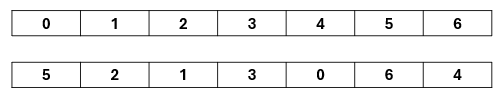
\includegraphics[width=0.8\textwidth]{
        papers/variationsprinzip_algorithmen/images/teil2/02_genetic_string_cities.png
        }
	\caption{Beispiel von Stätten in einem Genetic String dargestellt}
	\label{fig:cities_genetic_string}
\end{figure}


in Geld 2 wird immer die Farbe Grün angezeigt,  Ausserdem ändern nicht die Reihenfolge
der der Stätte, wodurch bei änderungen nicht nur die Position 
Bei den Stätten ist dies nicht einfach so umzusetzen da Bei einem Rucksack, welches einzelne Gegenstände hat 


